\chapter{Introduction}\label{sec:introduction}
The field of music information retrieval has seen many successes since the emergence of deep learning.
Supervised, end-to-end learning methods have been widely used in tasks like chord recognition \cite{korzeniowski_fully_2016, chen_harmony_2019}, key detection \cite{korzeniowski_end--end_2017}, beat tracking \cite{bock_joint_2016}, music audio tagging \cite{pons_end--end_2017} and music recommendation \cite{van_den_oord_deep_2013}.
These methods use labeled corpora, which are hard \cite{doi:10.1080/09298215.2019.1613436}, expensive and time-consuming to create, while raw unlabeled musical data is available in vast amounts.
Despite the importance of unsupervised learning in MIR for raw, high-dimensional signals of audio, it has yet to see breakthroughs similar to supervised learning.
It has enjoyed successes with methods like PCA, PMSC's and spherical $k$-means that rely on a transformation pipeline \cite{hamel2011temporal, dieleman_feature_learning}, but learning effective representations of raw audio remains elusive.

\begin{figure}[t]
    \centering
    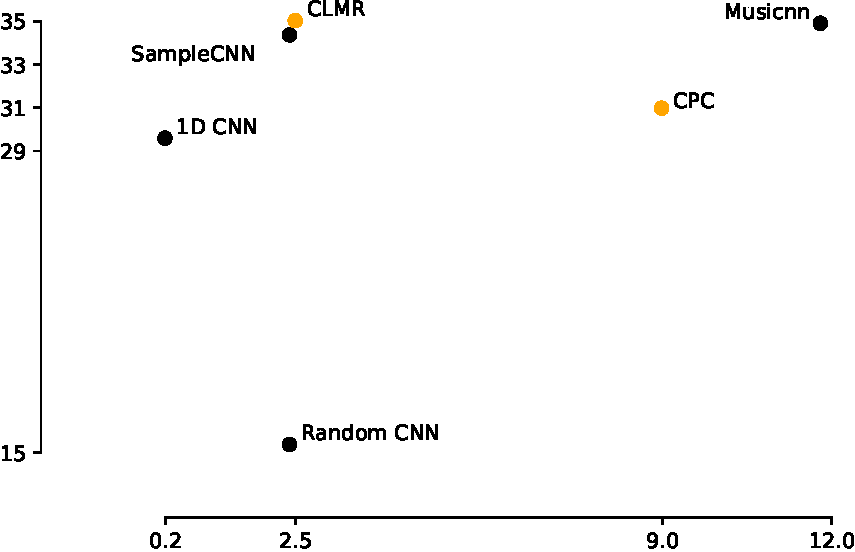
\includegraphics[width=0.75\columnwidth]{figs/roc_auc_magnatagatune.pdf}
    \caption{Performance and model complexity comparison of supervised models (grey) and self-supervised models (ours) in music classification of raw audio waveforms on the MagnaTagATune dataset to evaluate musical representations.
Supervised models were trained end-to-end, while CLMR and CPC are pre-trained without ground truth: their scores are obtained by training a linear classifier on their learned representations but nonetheless perform practically identically to the supervised models.}
    \label{fig:example}
\end{figure}

Self-supervised representation learning, a form of unsupervised learning, is a relatively new, upcoming learning paradigm \cite{dosovitskiy2015discriminative, oord_representation_2019, hjelm_learning_2019,chen_simple_2020}.
The general goal of representation learning is to train a function $g$ that maps input data $x \in \mathbb{R}^d$ to some representation of lower dimensionality, while preserving as much useful information as possible.
In the absence of ground truth, there can be no ordinary loss function for training $g$; self-supervised learning trains by way of a proxy loss function instead, obtained by withholding or augmenting parts of the input data.
One way to preserve the amount of useful information during self-supervised learning is to define the proxy loss function with respect to a relatively simple `pretext' task, with the idea that a representation that is good for the pretext task will also be useful for other tasks.
Many approaches simply rely on heuristics to design pretext tasks \cite{doersch_unsupervised_2015,zhang2016colorful}, e.g., by defining pitch transformation as a pretext task \cite{spice}.
Alternatively, \emph{contrastive representation learning} formulates the proxy loss directly on the learned representations and relies on comparing and contrasting multiple, slightly differing versions of any one example.
The rationale behind this contrastive strategy is \emph{predictive coding}, a theory that the human brain encodes causal structures and predicts future events at different levels of abstraction \cite{friston_predictive_2009}.


% may want to zoom out a bit, from 50 - 100 y-axis
% put in parenthesis [ours]
% square brackets citation
% add random baseline at 60% ROC
% add a labeled bracket that indicates the penalty / cost -> self-supervision penalty
% make the point of self-supervised learning this way

In this paper, we transfer the SimCLR framework \cite{chen_simple_2020} to the raw audio domain and contribute a pipeline of data augmentations on raw audio to form a simple framework for self-supervised, contrastive  learning of representations of raw audio waveforms.
To compare the effectiveness of this simple framework compared to a more complex self-supervised learning objective, we also evaluate representations learned by contrastive predictive coding \cite{oord_representation_2019}.
The models are evaluated on the downstream music tagging task, enabling us to evaluate their versatility: music tags describe many characteristics of music, e.g., genre, instrumentation and dynamics.
Our key contributions are summarized as follows.
\begin{itemize}
    \item CLMR achieves strong performance on the music classification task, despite self-supervised pre-training and fine-tuning on the downstream task using a linear classifier (see Figure~\ref{fig:example}).
    \item CLMR learns useful, compact representations from raw signals of musical audio.
    \item The learned representations are transferable across different musical corpora.
    \item CLMR can learn from \emph{any} dataset of raw audio, requiring neither transformations nor fine-tuning on the input data; nor do the models require manually annotated labels for pre-training.
    \item We provide an ablation study on the effectiveness of the data augmentations of raw audio.
\end{itemize}


\section{Outline}
In the following chapter, a comprehensive background of the field of self-supervised learning is be presented, as well as common neural network architectures in the raw audio domain.
Subsequently, the main downstream task and application of this thesis will be elaborated upon, along with its evaluation metrics.

In chapter 3, the method of this thesis is presented, outlining the details of the architecture of the model, its intuition, the objective function and the evaluation of the performance of the model.

In chapter 4, the implementation of the framework is discussed.

In chapter 5, the datasets are outlined, both for the main and transfer learning experiments.

In chapter 6, the results of this thesis are presented [...].

Lastly, the conclusions of this thesis are presented in chapter 9.

